\documentclass[12pt]{article}

\usepackage{sbc-template}
\usepackage{graphicx,url}
\usepackage[utf8]{inputenc}
\usepackage[brazil]{babel}
\usepackage{booktabs}
\usepackage{multirow}
\usepackage{amsmath}
\usepackage{amssymb}

\sloppy

\title{Avaliação Semântica de Super-Resolução Temporal em\\
       Imagens Sentinel-2 por Métricas de Processamento\\
       de Linguagem Natural}

\author{Marcel Fernandes Gomes\inst{1}}

\address{Instituto de Informatica – Universidade Federal do Rio Grande do Sul (UFRGS)\\Porto Alegre – RS – Brasil
  \email{marcelgfernandes@gmail.com}
}

\begin{document}

\maketitle

\begin{abstract}
Super-resolution (SR) recovers high-frequency detail from low-resolution
satellite imagery, but assessing whether the recovered content is
\emph{semantically} meaningful remains open. This work proposes a pipeline
that uses Natural Language Processing (NLP) metrics and vision-language
models to evaluate the semantic quality of super-resolved Sentinel-2
images, without pixel-wise metrics. Low-resolution (LR, $\approx$11.5~m/px)
and super-resolved (SR, $\approx$2.4~m/px) patches are captioned with BLIP
and GeoChat and scored with BLEU-1, ROUGE-1, TF-IDF cosine similarity,
CLIPScore (generic CLIP and RemoteCLIP) and a stratified Visual Question
Answering (VQA) protocol. The central contribution maps VQA land-cover
estimates onto a vector ground truth, eliminating lexical dependence and
yielding an interpretable error in percentage points: SR cuts the global
estimation error from $22.7$ to $19.1$~pp, with the largest gains in bare
soil ($+11.1$~pp) and agriculture ($+6.3$~pp). Validated on \textbf{two
geographically distinct regions} (953 pooled tiles), RemoteCLIP
image-image gains reach $+0.51$ (952/953 tiles), confirming a robust and
consistent semantic improvement.
\end{abstract}

\begin{resumo}
Técnicas de super-resolução (SR) recuperam detalhes de alta frequência
em imagens de satélite de baixa resolução, mas avaliar se o conteúdo
recuperado é \emph{semanticamente} relevante permanece um problema em
aberto. Este trabalho propõe um pipeline que usa métricas de
Processamento de Linguagem Natural (PLN) e modelos visão-linguagem para
mensurar a qualidade semântica de imagens Sentinel-2 super-resolvidas,
sem métricas por pixel. Recortes de baixa resolução
(LR, $\approx$11,5~m/px) e super-resolvidos (SR, $\approx$2,4~m/px) são
legendados por BLIP e GeoChat e pontuados por BLEU-1, ROUGE-1, cosseno
TF-IDF, CLIPScore (CLIP genérico e RemoteCLIP) e um protocolo de
\textit{Visual Question Answering} (VQA) estratificado. A contribuição
central mapeia as estimativas de cobertura do solo do VQA contra um ground
truth vetorial, eliminando a dependência léxica e gerando um erro
interpretável em pontos percentuais: a SR reduz o erro global de
$22{,}7$ para $19{,}1$~pp, com maiores ganhos em solo exposto
($+11{,}1$~pp) e agricultura ($+6{,}3$~pp). Validado em \textbf{duas
regiões geograficamente distintas} (953 tiles combinados), os ganhos
RemoteCLIP imagem-imagem chegam a $+0{,}51$ (952/953 tiles), confirmando
uma melhora semântica robusta e consistente.
\end{resumo}


% ==========================================================================
\section{Introdução}
% ==========================================================================

O monitoramento terrestre por satélite depende fortemente da resolução
espacial dos sensores. O Sentinel-2 (Agência Espacial Europeia) oferece
cobertura global multitemporal com resolução nativa de 10~m/px nas bandas
de cor natural, o que limita a identificação de feições finas como bordas
de campos, pequenos corpos d'água e estruturas urbanas de menor porte.
Técnicas de super-resolução (SR) por aprendizado profundo reconstroem
imagens de resolução mais alta a partir de múltiplas observações
temporais de baixa resolução \cite{dong:2016,nguyen:2021}.

Um desafio central é a \textit{avaliação} das imagens super-resolvidas.
Métricas tradicionais como PSNR e SSIM operam em nível de pixel e medem
fidelidade fotométrica, mas não capturam se o conteúdo semântico
recuperado é coerente com a realidade do terreno: uma imagem SR pode ter
PSNR alto e ainda introduzir texturas incorretas que confundem sistemas
de classificação. Modelos de visão-linguagem como CLIP \cite{radford:2021}
e BLIP \cite{li:2022} abrem uma alternativa que consiste em avaliar imagens por meio
de linguagem natural e o CLIPScore \cite{hessel:2021} formaliza essa
ideia como similaridade entre embeddings de imagem e texto.

Este trabalho investiga a questão: \textbf{as imagens Sentinel-2
super-resolvidas por fusão temporal recuperam conteúdo semântico
mensurável frente às versões de baixa resolução, quando avaliadas por
métricas de PLN e modelos visão-linguagem?} As contribuições são:
(i)~o uso de CLIPScore como métrica \emph{comparativa} entre resoluções,
sem exigir par de alta resolução perfeitamente alinhado;
(ii)~a substituição do BLIP genérico pelo GeoChat
\cite{kuckreja:2024}, especializado em sensoriamento remoto, sob uma
avaliação VQA estratificada em três níveis de sensibilidade à resolução;
(iii)~a contribuição central: uma avaliação cruzada entre as estimativas
de cobertura do solo do VQA e um ground truth vetorial (GeoPackage), que
elimina a dependência léxica e produz uma métrica quantitativa
interpretável em pontos percentuais; e (iv)~a validação do pipeline em
\textbf{duas regiões geograficamente distintas} do Sul do Brasil,
confirmando que os ganhos semânticos são consistentes entre paisagens
distintas e revelando modos de falha específicos à composição da
paisagem.


% ==========================================================================
\section{Referencial Teórico}
% ==========================================================================

\textbf{Super-resolução de satélite.} SR é o problema inverso de estimar
uma imagem de alta resolução a partir de uma ou mais de baixa resolução
\cite{dong:2016}. A abordagem multitemporal explora o fato de que o
satélite revisita a mesma área periodicamente: variações sub-pixel entre
observações carregam informação complementar que, combinada, reconstrói
detalhes abaixo da resolução nativa \cite{nguyen:2021}.

\textbf{Legendagem de imagens.} BLIP (\textit{Bootstrapping
Language-Image Pre-training}) \cite{li:2022} gera descrições textuais a
partir de imagens. Pré-treinado em pares imagem-texto da Web, produz
legendas de vocabulário diversificado, mas genérico. GeoChat
\cite{kuckreja:2024}, ao contrário, é um modelo visão-linguagem
(arquitetura LLaVA, encoder CLIP, decodificador LLaMA-7B) \textit{fine-tuned}
em 318~mil pares de instrução geoespaciais, cobrindo legendagem,
localização e VQA sobre imagens de satélite, o que o torna mais
discriminativo no domínio.

\textbf{Embeddings visão-linguagem.} CLIP \cite{radford:2021} aprende um
espaço latente compartilhado entre imagem e texto por \textit{contrastive
learning}; a similaridade cosseno nesse espaço mede alinhamento
semântico. RemoteCLIP \cite{liu:2024} especializa o CLIP para
sensoriamento remoto (datasets RSICD, RSITMD, UCM), desenvolvendo
representações mais discriminativas para classes de cobertura do solo.

\textbf{Métricas de PLN.} \textit{BLEU-1} \cite{papineni:2002} mede
precisão de unigramas (correspondência léxica). \textit{ROUGE-1}
\cite{lin:2004} combina revocação e precisão de unigramas via F1.
A \textit{similaridade cosseno TF-IDF} representa cada texto como vetor
TF-IDF e, pelo IDF, atenua o peso de termos muito frequentes, focando
nos discriminativos; como toda representação léxica, porém, não captura
sinonímia. Para superar essa dependência léxica, a \textit{similaridade
semântica} emprega um modelo Sentence-BERT (SBERT) \cite{reimers:2019},
que projeta sentenças em um espaço vetorial onde o cosseno reflete
proximidade de significado. O \textbf{CLIPScore}
\cite{hessel:2021} é definido como
\begin{equation}
  \text{CLIP-S}(c, v) = w \cdot \max\!\left(\cos\!\left(\mathbf{e}_c,\, \mathbf{e}_v\right),\, 0\right),
\end{equation}
onde $\mathbf{e}_c$ e $\mathbf{e}_v$ são os embeddings de texto e imagem
e $w=2{,}5$ é um fator de escala. Pode operar no modo imagem-texto ou
imagem-imagem (comparando duas imagens no espaço semântico).


% ==========================================================================
\section{Trabalhos Relacionados}
% ==========================================================================

A avaliação de qualidade de SR é historicamente dominada por métricas de
distorção como PSNR e SSIM \cite{wang:2004}, hoje reconhecidas como
fracamente correlacionadas com a percepção humana e com o desempenho em
tarefas \textit{downstream} \cite{blau:2018}. Blau e Michaeli (2018)
formalizaram o \textit{perception-distortion tradeoff}, mostrando que
melhorar a qualidade perceptual frequentemente piora a fidelidade de
pixel, o que motiva métricas alternativas. No domínio de sensoriamento
remoto, Nguyen et al.\ \cite{nguyen:2021} propõem um benchmark de SR
multitemporal para Sentinel-2 avaliado por PSNR/SSIM contra imagens de
alta resolução; o presente trabalho difere por usar linguagem natural
como referência semântica, dispensando um par HR perfeitamente alinhado.

A legendagem de imagens de sensoriamento remoto foi explorada em datasets
como RSICD \cite{lu:2017}, com modelos do tipo BLIP. Hessel et al.\
\cite{hessel:2021} introduziram o CLIPScore como avaliação
referência-livre com alta correlação humana, e Liu et al.\ \cite{liu:2024}
o estenderam ao domínio aéreo com o RemoteCLIP. Diferentemente desses
trabalhos, aqui o CLIPScore é usado como métrica \emph{comparativa entre
resoluções} (LR vs.\ SR), e a etapa de avaliação cruzada VQA $\times$
GeoPackage elimina a dependência léxica ao substituir a comparação
textual por uma métrica quantitativa de estimativa de cobertura do solo.
A validade dos ganhos é confirmada em \emph{múltiplas regiões}, e não em
uma única cena.


% ==========================================================================
\section{Metodologia}
% ==========================================================================

A Tabela~\ref{tab:pipeline_overview} resume os modelos, métricas e
cenários combinados ao longo do trabalho. O mesmo pipeline é executado
independentemente em duas regiões.

\begin{table}[ht]
\centering
\caption{Visão geral do pipeline: modelos, métricas e cenários.
  \checkmark\,=\,aplicado; e -\,=\,não aplicado.}
\label{tab:pipeline_overview}
\small
\begin{tabular}{llccc}
\toprule
\textbf{Modelo} & \textbf{Métrica / Modo} & \textbf{Cen.\,A} & \textbf{Cen.\,B} & \textbf{Cen.\,C} \\
\midrule
\multirow{2}{*}{BLIP}
  & NLP (BLEU, ROUGE, TF-IDF)           & \checkmark & \checkmark & \checkmark \\
  & CLIPScore img$\leftrightarrow$texto & \checkmark & ---        & ---        \\
\midrule
(sem modelo)
  & CLIPScore img$\leftrightarrow$img$^\dagger$ & --- & \checkmark & \checkmark \\
\midrule
\multirow{3}{*}{GeoChat}
  & NLP (BLEU, ROUGE, TF-IDF)           & ---        & \checkmark & ---        \\
  & VQA estratificada (7 perguntas)      & \checkmark & ---        & ---        \\
  & VQA $\times$ GeoPackage (MAE q01)   & \checkmark & ---        & ---        \\
\bottomrule
\multicolumn{5}{l}{\footnotesize $^\dagger$O modo img$\leftrightarrow$img extrai embeddings visuais de LR, SR e GT} \\
\multicolumn{5}{l}{\footnotesize \hspace{1em}diretamente pelo encoder CLIP, sem modelo de legendagem.} \\
\end{tabular}
\end{table}

\subsection{Dados e Regiões}

As entradas são cenas Sentinel-2 (canal TCI, composição RGB das bandas
4-3-2), no Sul do Brasil. A imagem de baixa resolução (\textbf{LR}) tem
$\approx$11,5~m/px; a super-resolvida (\textbf{SR}) é o produto
\textit{blended} por fusão temporal de 8 observações, a $\approx$2,4~m/px.
O ground truth raster (\textbf{GT}) é uma ortofoto aérea de $\approx$1~m/px;
o ground truth vetorial é um GeoPackage com 7 camadas de cobertura do solo
(floresta, campo, massa d'água, terreno exposto, brejo/pântano, vegetação
cultivada, área edificada), de anotação manual.

Para validar a robustez do pipeline, o experimento é replicado em
\textbf{duas regiões geograficamente distintas} ($\approx$110~km de
distância em EPSG:3857): \textbf{Região~1} ($n=575$ tiles válidos) e
\textbf{Região~2} ($n=378$ tiles), totalizando \textbf{953 tiles}
combinados. As regiões diferem em composição de paisagem, a Região~2 é
mais agrícola e tem corpos d'água raros e pequenos, o que permite
identificar tanto a consistência dos ganhos entre paisagens como modos
de falha específicos à composição local.

\subsection{Reprojeção, Tiling e Atribuição de Classe}

Todas as imagens são reprojetadas para EPSG:3857 (Rasterio). O GT é
carregado em duas versões: original ($\approx$1~m/px) e reamostrado
bilinearmente para $\approx$2,4~m/px (resolução da SR). As imagens são
particionadas em um grid de tiles de 64$\times$64 px no espaço LR
($\approx$0,73~km²/tile); tiles com $>$50\% de NoData são descartados.
Para cada tile, os polígonos vetoriais são intersectados com sua
\textit{bounding box}; a classe dominante é atribuída quando a interseção
supera 5\% da área. Na Região~1, 437/575 tiles têm classe dominante
(Cenário A); na Região~2, todos os 378.

\subsection{Cenários e Métricas}

Definem-se três cenários de referência:
\textbf{(A) GT Vetorial} com referência = nome da classe em inglês;
\textbf{(B) GT Raster 1m} com referência = legenda BLIP da ortofoto (NLP)
ou embedding da ortofoto (CLIPScore imagem-imagem);
\textbf{(C) GT Raster Reamostrado}, idêntico a B, com GT degradado para
$\approx$2,4~m/px, isolando a penalidade de resolução diferencial.

As métricas NLP são BLEU-1 (suavização \textit{method1}, NLTK), ROUGE-1
F1 e cosseno TF-IDF. O CLIPScore usa \texttt{clip-vit-base-patch32}
(genérico) e \texttt{RemoteCLIP-ViT-B-32}, com $w=2{,}5$ sobre embeddings
normalizados. As legendas livres são geradas por
\texttt{blip-image-captioning-base} e, no Cenário~B, também pelo GeoChat-7B
(FP16 em V100, ou NF4 de 4~bits em GPUs menores), permitindo comparação
direta entre os dois modelos.

\subsection{VQA Estratificada}

Legendas livres saturam quando o modelo descreve bem ambas as resoluções.
Para isolar o que a resolução muda, o GeoChat é consultado com 7 perguntas
objetivas em 3 níveis: \textbf{L1 -- Semântico} (q01 estimativa percentual
de classes; q02 presença de água); \textbf{L2 -- Estrutural} (q03 contagem
de campos; q04 fileiras de cultivo); \textbf{L3 -- Detalhe fino} (q05--q07
contagem/descrição de edifícios e vias). A hipótese é que L3 favoreça mais
a SR. As respostas LR, SR e GT são comparadas par a par por cosseno TF-IDF,
similaridade semântica (SBERT, \texttt{all-MiniLM-L6-v2}) e, para q01, MAE em
pontos percentuais (pp).

\subsection{Avaliação Cruzada VQA $\times$ GeoPackage}
\label{sec:vqa_vetorial_met}

Para contornar a incompatibilidade léxica do Cenário~A, as respostas de
q01 são usadas como predições e o GeoPackage como ground truth
quantitativo. Para cada tile: (i) as camadas vetoriais são intersectadas
com sua \textit{bbox} e agregadas em 5 classes VQA, \textit{forest},
\textit{agriculture} (campo\,+\,vegetação cultivada), \textit{urban},
\textit{water}, \textit{bare soil} (terreno exposto\,+\,brejo); (ii) as
estimativas percentuais de q01 (LR, SR, GT) são parseadas; (iii) calcula-se
o MAE por classe e global. Isso substitui a comparação textual por uma
quantitativa, interpretável em pp e comparável entre resoluções.


% ==========================================================================
\section{Experimentos e Resultados}
% ==========================================================================

Os experimentos usam Python 3.13, PyTorch 2.x, Transformers 5.x,
open\_clip\_torch 2.x e Rasterio 1.3. As etapas BLIP rodam em CPU; as
etapas GeoChat em GPU Tesla V100-32GB (FP16) e, localmente, em Quadro
RTX~4000 (NF4). Os resultados são reportados por região (R1, R2) e
combinados (pooled, $n=953$), de modo que a coluna pooled mede o
comportamento agregado e a comparação R1\,vs.\,R2 mede a robustez.
A direção das diferenças LR\,vs.\,SR é resumida pela fração de tiles em
que SR\,$>$\,LR (coluna SR\,$>$\,LR das tabelas): nas métricas principais
essa fração é largamente majoritária (p.\,ex.\ 952/953 no RemoteCLIP
imagem-imagem), indicando que os ganhos são consistentes entre tiles e
não atribuíveis a poucos casos extremos.

\subsection{Cenário A: limitação léxica}

No Cenário~A, os scores NLP ficam próximos de zero em ambas as resoluções
e regiões (TF-IDF SR $\approx 0{,}02$--$0{,}03$; SR\,$>$\,LR em apenas
71/815 tiles combinados), pois o BLIP raramente reproduz literalmente o
nome da classe. A análise qualitativa explica o piso da LR: 20\% dos tiles
LR da Região~1 geram descrições alucinadas, medido no Cenário~B, como
legendas com BLEU-1\,$\approx$\,0 frente à ortofoto (p.\,ex.\ \textit{``a
blue sky with clouds''}, \textit{``a couple is kissing in the water''}),
pois a resolução insuficiente leva o BLIP a evocar cenas do seu
pré-treinamento; a SR reduz esse colapso para 11\%. Esse cenário motiva a avaliação cruzada
quantitativa da Seção~\ref{sec:vqa_vetorial}.

\subsection{Cenários B e C: CLIPScore e NLP imagem-imagem}

O CLIPScore imagem-imagem (Cenário~B) é o resultado mais expressivo e o
mais \emph{estável} entre regiões (Tabela~\ref{tab:clip_gt1m}). O
RemoteCLIP classifica a SR como mais próxima da ortofoto em
\textbf{952/953} tiles ($\Delta=+0{,}508$ pooled), com ganho praticamente
idêntico em R1 ($+0{,}505$) e R2 ($+0{,}512$). O CLIP genérico confirma a
direção com magnitude menor, indicando que o modelo especializado captura
melhor as diferenças de qualidade relevantes ao domínio. As métricas NLP
do BLIP (Cenário~B) também favorecem a SR de forma consistente nas duas
regiões: BLEU-1 $\Delta=+0{,}157$, ROUGE-1 $+0{,}189$ e TF-IDF $+0{,}201$
(pooled), com 657--700/953 tiles favoráveis. No Cenário~C (GT
reamostrado), os ganhos NLP se mantêm ($\Delta_{\text{TF-IDF}}=+0{,}227$),
enquanto o gap RemoteCLIP comprime de $+0{,}508$ para $+0{,}421$: parte da
vantagem medida pelo CLIP é penalidade de resolução, mas a hierarquia
LR\,$<$\,SR persiste mesmo após equalizar as resoluções.

\begin{table}[ht]
\centering
\caption{CLIPScore imagem-imagem (Cenário~B) e NLP-BLIP (Cenário~B) por
  região e combinado. $\Delta = $ SR\,$-$\,LR.}
\label{tab:clip_gt1m}
\small
\begin{tabular}{llcccc}
\toprule
\textbf{Métrica} & \textbf{Região} & \textbf{LR} & \textbf{SR} & \textbf{$\Delta$} & \textbf{SR$>$LR} \\
\midrule
\multirow{3}{*}{CLIP genérico}
  & R1     & 1{,}846 & 2{,}203 & $+$0{,}356 & 562/575 \\
  & R2     & 1{,}880 & 2{,}225 & $+$0{,}345 & 368/378 \\
  & pooled & 1{,}860 & 2{,}211 & $+$0{,}352 & 930/953 \\
\midrule
\multirow{3}{*}{RemoteCLIP}
  & R1     & 1{,}543 & 2{,}048 & $+$0{,}505 & 574/575 \\
  & R2     & 1{,}515 & 2{,}027 & $+$0{,}512 & 378/378 \\
  & pooled & 1{,}532 & 2{,}040 & $\mathbf{+0{,}508}$ & \textbf{952/953} \\
\midrule
\multirow{3}{*}{BLIP TF-IDF}
  & R1     & 0{,}077 & 0{,}286 & $+$0{,}209 & 403/575 \\
  & R2     & 0{,}081 & 0{,}269 & $+$0{,}188 & 282/378 \\
  & pooled & 0{,}079 & 0{,}279 & $+$0{,}201 & 685/953 \\
\bottomrule
\end{tabular}
\end{table}

\subsection{GeoChat: legendas livres e VQA estratificada}

Substituir o BLIP pelo GeoChat eleva os scores absolutos (TF-IDF SR de
$0{,}279$ para $0{,}769$ pooled) e \emph{reduz} o gap relativo
($\Delta_{\text{TF-IDF}}=+0{,}099$): o GeoChat descreve bem também a LR e
não alucina, confirmando que o ganho da SR é real e que o BLIP inflava o
gap ao colapsar na LR. Notavelmente, os ganhos GeoChat são \emph{maiores}
na Região~2 (BLEU-1 $+0{,}120$ vs.\ $+0{,}086$ em R1), indicando que a
paisagem mais agrícola da R2 se beneficia mais da SR na legendagem.

A VQA estratificada (Tabela~\ref{tab:vqa_nivel}) favorece a SR em todos os
níveis e nas duas regiões. O nível semântico (L1) tem o maior ganho
TF-IDF ($+0{,}228$ pooled), puxado por q02 (presença de água,
$\Delta=+0{,}386$) e q01. Em q01, tomando como referência a própria
resposta do GeoChat sobre a ortofoto (GT raster), e não o GeoPackage da
Seção~\ref{sec:vqa_vetorial} ---, a SR reduz o MAE de estimativa de
cobertura de $11{,}83$ para $6{,}30$~pp (pooled), uma melhora de
$1{,}9\times$. O nível estrutural (L2) é o mais fraco: q03 (contagem de
campos) satura em zero em ambas as resoluções, inadequada à escala dos
tiles. Em todos os níveis, R2 apresenta ganhos iguais ou superiores a R1.

\begin{table}[ht]
\centering
\caption{VQA estratificada: ganho $\Delta$(SR$-$LR) em TF-IDF e
  similaridade semântica, por nível e região. $n$ = pares de resposta.}
\label{tab:vqa_nivel}
\small
\begin{tabular}{llccc}
\toprule
\textbf{Nível} & \textbf{Região} & \textbf{$n$} & \textbf{TF-IDF $\Delta$} & \textbf{Sem.\ $\Delta$} \\
\midrule
\multirow{3}{*}{L1 Semântico}
  & R1 & 1150 & $+$0{,}223 & $+$0{,}052 \\
  & R2 &  756 & $+$0{,}236 & $+$0{,}056 \\
  & pooled & 1906 & $+$0{,}228 & $+$0{,}054 \\
\midrule
\multirow{3}{*}{L2 Estrutural}
  & R1 & 1150 & $+$0{,}115 & $+$0{,}039 \\
  & R2 &  756 & $+$0{,}156 & $+$0{,}052 \\
  & pooled & 1906 & $+$0{,}131 & $+$0{,}044 \\
\midrule
\multirow{3}{*}{L3 Detalhe fino}
  & R1 & 1725 & $+$0{,}099 & $+$0{,}040 \\
  & R2 & 1134 & $+$0{,}156 & $+$0{,}081 \\
  & pooled & 2859 & $+$0{,}122 & $+$0{,}056 \\
\bottomrule
\end{tabular}
\end{table}

\subsection{VQA $\times$ GeoPackage: avaliação cruzada com ground truth vetorial}
\label{sec:vqa_vetorial}

A Tabela~\ref{tab:vqa_vetorial} cruza as estimativas de q01 com os
percentuais reais do GeoPackage. Globalmente, a SR estima a cobertura do
solo com erro $3{,}6$~pp menor que a LR (pooled), e a hierarquia
GT\,raster\,$<$\,SR\,$<$\,LR é consistente nas duas regiões
($17{,}4 < 19{,}1 < 22{,}7$~pp pooled), a SR recupera a maior parte do
sinal semântico relevante para estimativa de cobertura. Os maiores ganhos
ocorrem em \textit{bare soil} ($+11{,}1$~pp) e \textit{agriculture}
($+6{,}3$~pp) pooled, robustos em ambas as regiões
(Figura~\ref{fig:mae_multi}). A Figura~\ref{fig:grid} ilustra tiles
representativos das duas regiões, evidenciando a recuperação de detalhes
pela SR em diferentes tipos de paisagem.

\begin{table}[ht]
\centering
\caption{MAE (pp) de estimativa de cobertura vs.\ GeoPackage por classe,
  região e combinado. $\Delta=$LR$-$SR (positivo = SR melhor). Menor MAE
  é melhor. O MAE global usa os tiles cuja resposta de q01 tem formato
  parseável.}
\label{tab:vqa_vetorial}
\small
\resizebox{\textwidth}{!}{%
\begin{tabular}{lccc|ccc|ccc}
\toprule
& \multicolumn{3}{c|}{\textbf{Região 1} ($n{=}575$)}
& \multicolumn{3}{c|}{\textbf{Região 2} ($n{=}378$)}
& \multicolumn{3}{c}{\textbf{Pooled} ($n{=}953$)} \\
\textbf{Classe} & LR & SR & $\Delta$ & LR & SR & $\Delta$ & LR & SR & $\Delta$ \\
\midrule
forest      & 37{,}1 & 36{,}6 & $+$0{,}5 & 28{,}8 & 23{,}9 & $+$4{,}9 & 33{,}8 & 31{,}6 & $+$2{,}2 \\
agriculture & 30{,}4 & 26{,}1 & $+$4{,}3 & 50{,}1 & 41{,}0 & $+$9{,}2 & 38{,}3 & 31{,}9 & $+$6{,}3 \\
urban       &  5{,}1 &  3{,}7 & $+$1{,}4 &  5{,}0 &  5{,}8 & $-$0{,}9 &  5{,}1 &  4{,}5 & $+$0{,}5 \\
water       & 11{,}5 &  9{,}6 & $+$1{,}9 &  4{,}7 & 13{,}4 & $-$8{,}7 &  8{,}8 & 11{,}1 & $-$2{,}3 \\
bare soil   & 29{,}4 & 20{,}2 & $+$9{,}2 & 24{,}4 & 10{,}3 & $+$14{,}0 & 27{,}4 & 16{,}4 & $+$11{,}1 \\
\midrule
\textbf{Global} & 22{,}7 & 19{,}2 & $+$3{,}5 & 22{,}6 & 18{,}9 & $+$3{,}7 & 22{,}7 & 19{,}1 & $+$3{,}6 \\
GT raster       & \multicolumn{3}{c|}{17{,}7} & \multicolumn{3}{c|}{16{,}9} & \multicolumn{3}{c}{17{,}4} \\
\bottomrule
\end{tabular}%
}
\end{table}

\begin{figure}[ht]
\centering
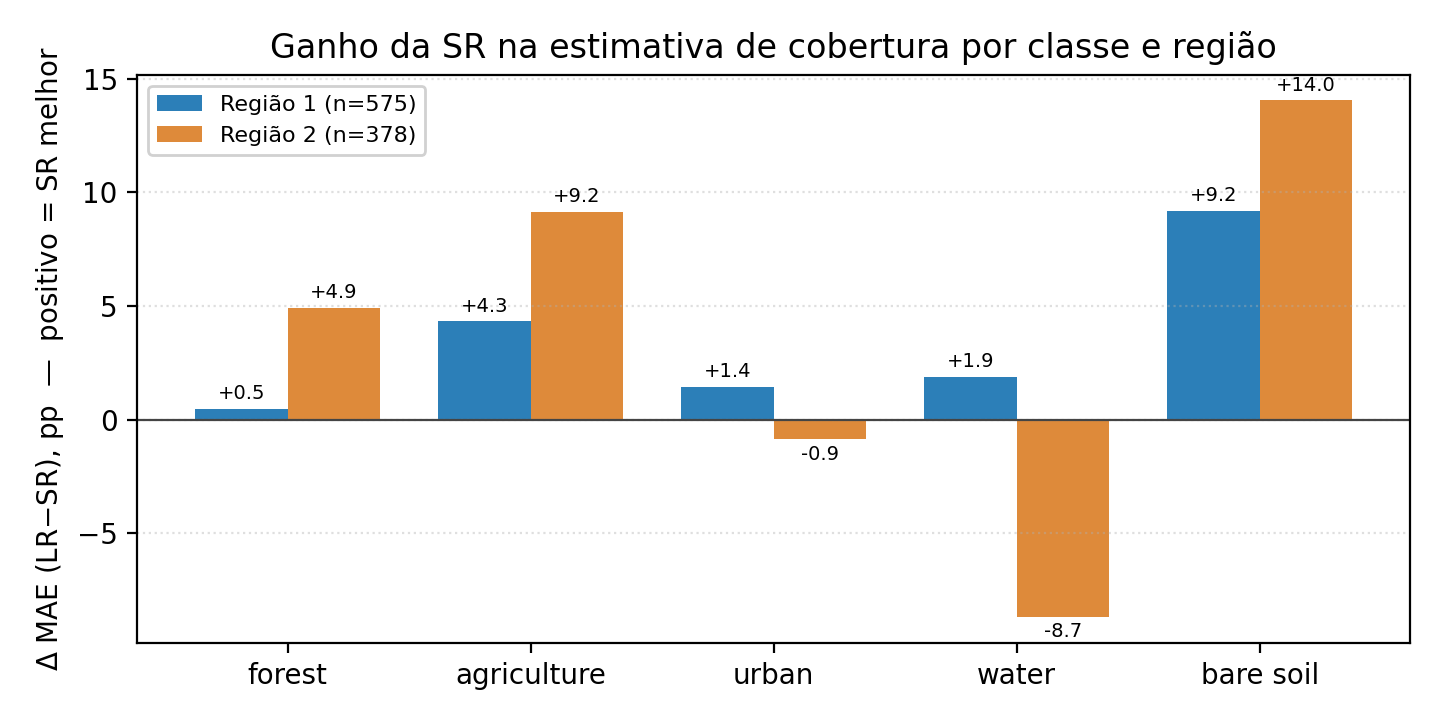
\includegraphics[width=.92\textwidth]{figures/fig_mae_multiregiao.png}
\caption{Ganho da SR ($\Delta$ MAE = LR$-$SR, em pp) na estimativa de
  cobertura por classe e região. Positivo = SR melhor. Os maiores ganhos
  ocorrem em \textit{bare soil} e \textit{agriculture}, robustos nas
  duas regiões.}
\label{fig:mae_multi}
\end{figure}

\begin{figure}[ht]
\centering
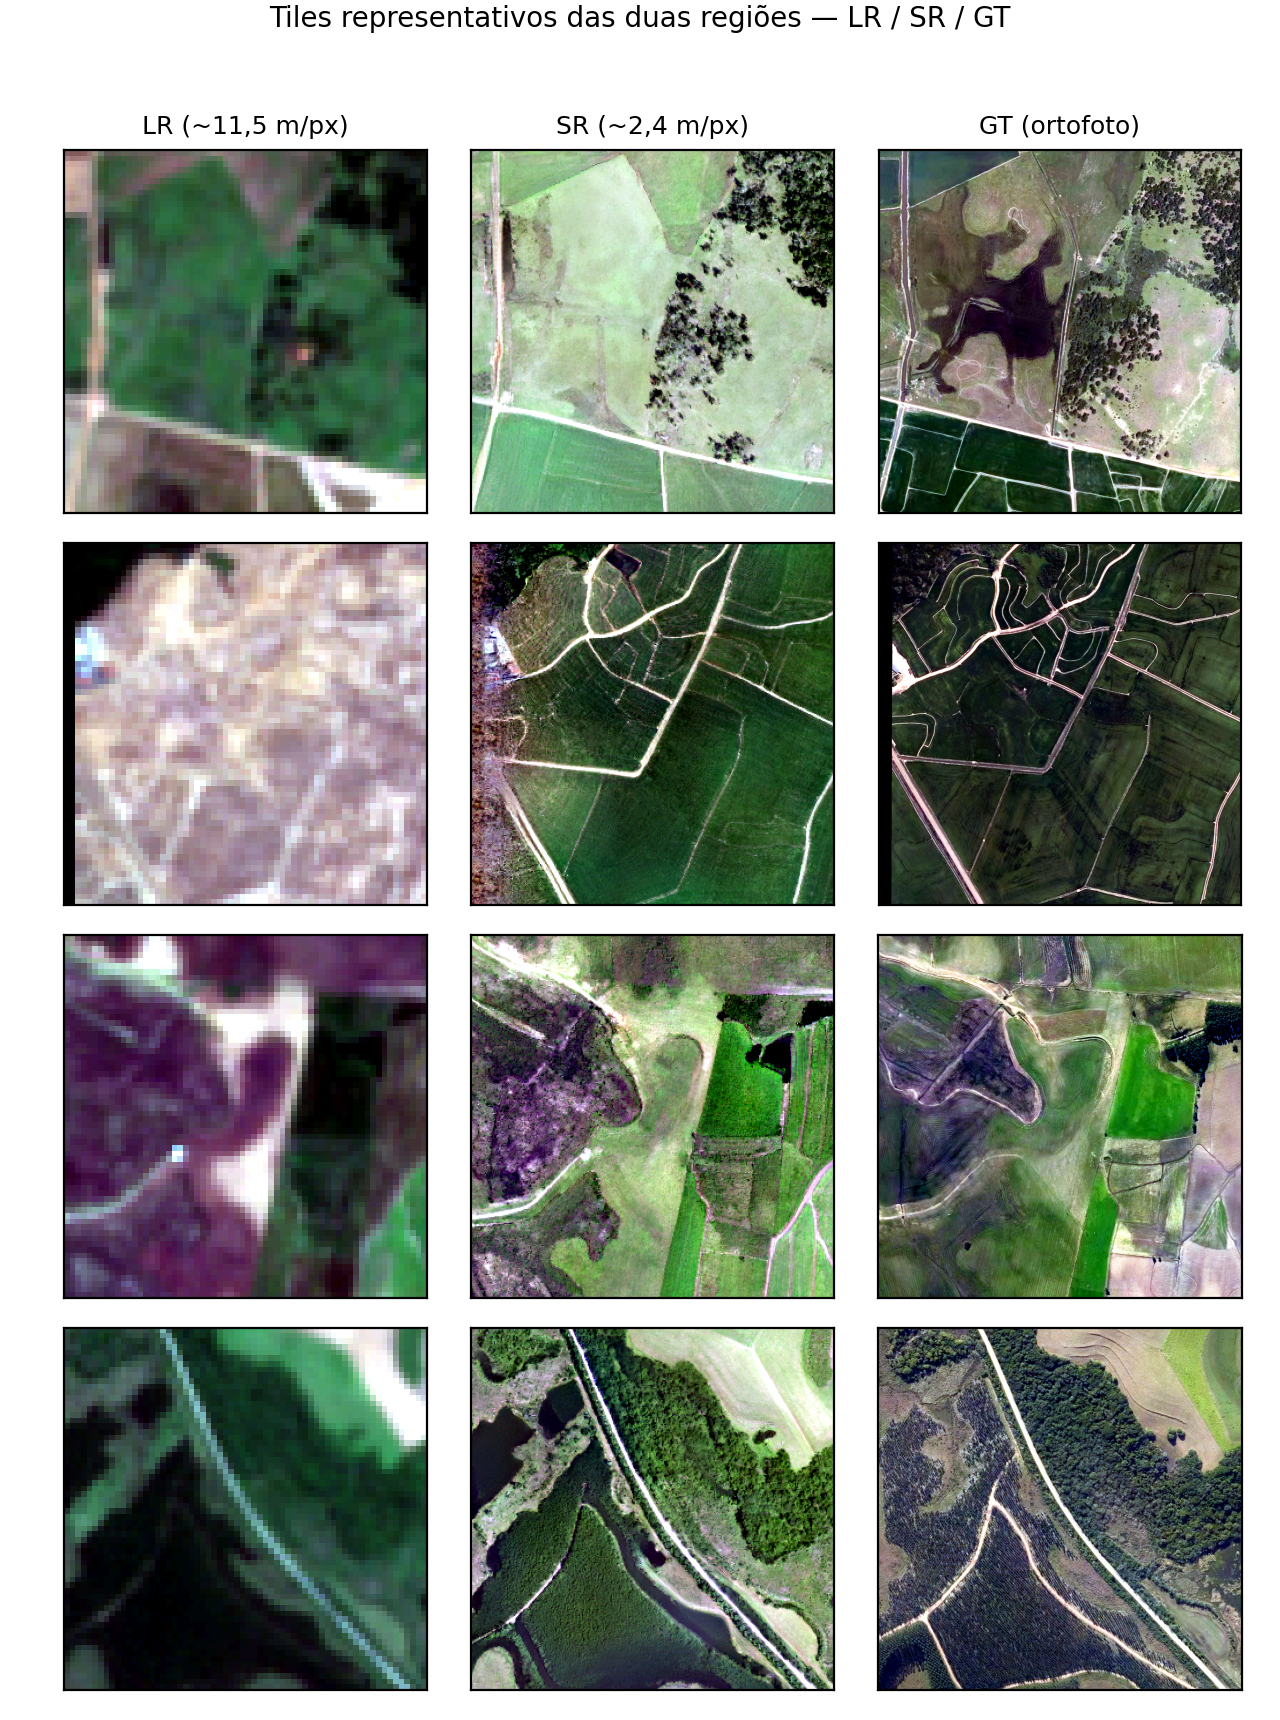
\includegraphics[width=.80\textwidth]{figures/fig_grid_representativo.png}
\caption{Tiles representativos das duas regiões (LR / SR / GT),
  ilustrando ganhos da SR: recuperação de detalhes de água,
  correção de solo exposto e melhora na descrição de áreas agrícolas.}
\label{fig:grid}
\end{figure}


% ==========================================================================
\section{Conclusão}
% ==========================================================================

Este trabalho avaliou, por métricas de PLN e modelos visão-linguagem, se
imagens Sentinel-2 super-resolvidas por fusão temporal recuperam conteúdo
semântico mensurável. O pipeline proposto vai além de métricas por pixel:
o CLIPScore RemoteCLIP imagem-imagem favorece a SR em 952/953 tiles
($\Delta=+0{,}508$), e as métricas NLP (BLIP e GeoChat) melhoram de forma
consistente. A contribuição central é a avaliação cruzada VQA $\times$
GeoPackage e fornece a evidência mais direta e interpretável: a SR reduz
o erro global de estimativa de cobertura do solo de $22{,}7$ para
$19{,}1$~pp ($-3{,}6$~pp) frente ao ground truth vetorial e, frente à
referência de alta resolução em q01, suas estimativas são $1{,}9\times$
mais precisas ($11{,}8\to6{,}3$~pp), sem depender de sobreposição léxica
ou de pares de alta resolução alinhados. Os maiores ganhos em
\textit{bare soil} ($+11{,}1$~pp) e \textit{agriculture} ($+6{,}3$~pp)
revelam que a fusão temporal recupera informação semântica real sobre
tipos de cobertura diretamente relevantes para monitoramento agrícola e
ambiental.

A validação em \textbf{duas regiões geograficamente distintas} (953 tiles
combinados) confirma a robustez dos resultados. Observou-se ainda que o
ganho semântico global pode coexistir com degradações específicas a certas
classes, por exemplo, na Região~2 (água rara) a SR tende a superestimar
a classe \textit{water}, uma nuance útil para calibrar expectativas por
tipo de paisagem.

Como trabalhos futuros: (i) ampliar para mais regiões, datas e condições
de nuvem, quantificando estatisticamente a variabilidade entre paisagens;
(ii) correlacionar as métricas semânticas com tarefas \textit{downstream}
(classificação, detecção); e (iii) reformular as perguntas VQA de nível
estrutural, que saturaram.

O código-fonte, os dados vetoriais e os resultados completos estão
disponíveis em: \texttt{https://github.com/MarcelFernandesCGEO/cmp617\_trabalho\_final}.

% ==========================================================================
\section*{Declaração de Uso de Inteligência Artificial Generativa}
% ==========================================================================

Declara-se o uso de ferramentas de IA generativa neste
trabalho. O modelo \textbf{Claude Opus 4.8 (Anthropic)}, via Claude Code
(versão 2.1.179), foi
utilizado para: (i) auxílio na consolidação e análise estatística dos
resultados das duas regiões (geração de scripts em Python/pandas);
(ii) geração de código de plotagem (matplotlib) das figuras consolidadas;
e (iii) revisão gramatical do texto. Os modelos
\textbf{BLIP}, \textbf{GeoChat}, \textbf{CLIP} e \textbf{RemoteCLIP}
constituem o objeto de estudo experimental, não ferramentas de redação.
Todo o conteúdo, contemplando código e texto, foi integralmente revisado,
validado e é de responsabilidade do autor. A concepção da pesquisa, o
desenho experimental multi-região e a interpretação dos achados são de
autoria própria.

\bibliographystyle{sbc}
\bibliography{artigo}

\end{document}
